\documentclass[10pt,twocolumn]{article}
\usepackage[a4paper,margin=0.72in,columnsep=0.25in]{geometry}
\usepackage[T1]{fontenc}
\usepackage{lmodern,microtype,graphicx,booktabs,amsmath,amssymb,amsthm,xcolor}
\usepackage{enumitem,listings,fancyhdr,url,xurl,array,balance}
\usepackage[font=small,labelfont=bf]{caption}
\usepackage[colorlinks=true,allcolors=teal!60!black,breaklinks=true]{hyperref}
\definecolor{ink}{HTML}{172B4D}
\definecolor{accent}{HTML}{008577}
\newtheorem{theorem}{Theorem}
\newtheorem{proposition}[theorem]{Proposition}
\newtheorem{definition}[theorem]{Definition}
\newcommand{\US}{\textsc{UndoScope}}
\newcommand{\ctx}{\mathsf{ctx}}
\newcommand{\head}{\mathsf{head}}
\newcommand{\rid}{\mathsf{id}}
\newcommand{\State}{\mathcal{S}}
\newcommand{\policy}{\mathsf{allow}}
\setlist{nosep,leftmargin=*}
\setlength{\parskip}{2pt}
\newcolumntype{L}[1]{>{\raggedright\arraybackslash}p{#1}}
\setlength{\emergencystretch}{1.5em}
\raggedbottom
\pagestyle{fancy}\fancyhf{}
\fancyhead[L]{\small\textcolor{ink}{UndoScope}}
\fancyhead[R]{\small Technical report \textbullet\ 23 September 2026}
\fancyfoot[C]{\thepage}\setlength{\headheight}{14pt}
\lstset{basicstyle=\ttfamily\footnotesize,breaklines=true,frame=single,rulecolor=\color{black!15},columns=fullflexible,showstringspaces=false}
\title{\vspace{-1.1em}\textbf{UndoScope: Effect-Scoped Compensation\\for Tool-Using Agents}}
\author{Shivam Gupta\\\small Independent Research\\\small\href{mailto:shivam1720406@gmail.com}{shivam1720406@gmail.com}}
\date{23 September 2026}
\begin{document}
\maketitle
\begin{abstract}
An agent can select the correct recovery tool and still damage another actor's work. A mapped inverse may overwrite an intervening assignment, remove an independently granted permission, or delete a resource that has changed since creation. We study \emph{recovery-effect isolation}: compensation may remove the recorded effect of an authorized workflow while preserving independent effects committed afterward. \US{} combines established compensation, provenance, version checks, and runtime authorization in a single-store reference contract for register assignments, additive contributions, tagged grants, and resource creation. Its contribution is an executable security specification and benchmark, rather than a new rollback primitive. An indistinguishability argument explains why current-value comparisons cannot provide both useful recovery and preservation of same-value peer writes. Across 1,364 bounded event histories, mapped inverses cause 521 collateral outcomes; \US{} causes none and completes all 678 recoveries admitted by the specified oracle. Object and component guards also avoid collateral mutation but complete 4 and 42 eligible recoveries. In 240 controlled model recovery tasks, paired execution of the same selected calls produces 60 collateral outcomes with mapped inverses and none with \US{}. Hardened GPT-4.1 selects no wrong receipts in its 60 tasks, yet mapped recovery still causes 15 collateral changes. Persistent SQLite experiments exercise concurrent retries and process death, and a working MCP adapter exposes only receipt-based recovery. The results identify operation-specific recovery semantics as a security boundary distinct from prompt robustness, with explicit limits for dependent workflows and external services.
\end{abstract}

\section{Introduction}
A support agent changes a ticket from \texttt{open} to \texttt{triage}. A downstream task fails, so the agent tries to undo its earlier change. Meanwhile, a support engineer has reviewed the ticket and independently confirmed \texttt{triage}. A compensator that checks whether the ticket still says \texttt{triage} and then restores \texttt{open} erases the engineer's decision. The receipt is genuine, the target is correct, and the inverse parameter is exactly the old value. The failure is in the semantics of recovery.

A similar ambiguity appears in access management. Two workflows independently grant the same contractor access. Canceling one workflow should remove its grant, while leaving the other grant effective. An inverse of the form ``revoke the contractor'' cannot express that distinction. In resource management, ``delete the object I created'' becomes unsafe when an operator modifies it, or when its name is reused for a different incarnation. These cases concern integrity and authority even when a model follows the user's request faithfully.

Compensation is a longstanding response to failures in long-running workflows \cite{sagas}. Its concurrency hazards are also established: Microsoft's architecture guidance explicitly distinguishes compensation from restoring an old snapshot \cite{azure}. Agent systems make the recovery boundary particularly visible because tool selection, error interpretation, and recovery requests may depend on untrusted text. Recent work supplies log-based compensation managers \cite{rac}, transaction-oriented planning \cite{sagallm}, and protections against replay after checkpoint restoration \cite{acrfence}. The remaining engineering question studied here is precise: \emph{what evidence must an individual compensating write check to avoid erasing independent work?}

We present \US{}, a reference contract and benchmark for answering this question. The model can request recovery by receipt identifier; a trusted adapter binds the request to a tenant, principal, and workflow, determines the inverse from the committed effect, and checks current authority and state inside the same transaction as the write. The operation-specific evidence varies. A register needs its provenance head; an additive effect needs its contribution identity and business invariant; a grant needs its unique tag; deleting a created resource needs its incarnation and unchanged revision.

The study separates three questions that aggregate recovery-success scores can conflate:
\begin{enumerate}
\item Is the requested effect inside the caller's current recovery authority?
\item Can its inverse preserve independently committed peer effects?
\item Did a permitted recovery actually complete, rather than merely return a reassuring response?
\end{enumerate}
A conservative implementation can answer the second question by rejecting every changed object. That is a useful safety baseline, but it loses recoveries that could preserve unrelated fields or independent additive contributions. Conversely, a permissive inverse can finish a workflow while corrupting peer state. Both axes must be measured.

Our contributions are: (i) a recovery-effect isolation contract with an explicit threat model and a provenance-necessity counterexample; (ii) a bounded, executable history benchmark with seven mechanism controls and guard ablations; (iii) paired model-tool experiments that separate selection failures from backend semantic failures; and (iv) a persistent SQLite implementation, crash/concurrency tests, and an MCP demonstrator. These are complementary to existing planners and recovery orchestrators. We do not evaluate an unmodified commercial agent or claim a new distributed transaction protocol.

\begin{figure}[t]
\centering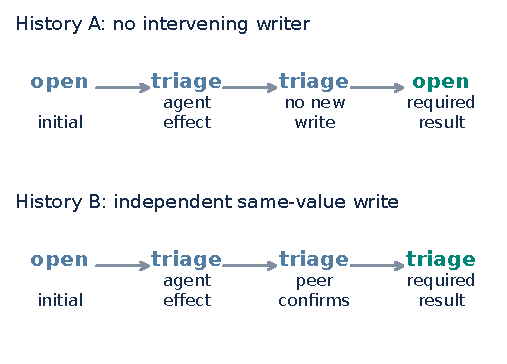
\includegraphics[width=\columnwidth]{figures/04-indistinguishable-values.pdf}
\caption{Identical current values can require different recovery decisions. A value-only guard observes the same old, written, and current values in both histories; provenance distinguishes the intervening writer.}
\label{fig:ambiguity}
\end{figure}

\section{Related work}
\paragraph{Compensation and selective undo.}
Sagas supply the foundational model of forward actions and compensations \cite{sagas}. Application-specific compensation, concurrency awareness, and idempotent recovery are documented engineering practice \cite{azure}. Origin-scoped selective undo is implemented by Yjs \cite{yjs}. Unique contributions and tagged sets have direct antecedents in replicated data types \cite{crdt}. \US{} uses these ideas in a recovery authorization boundary; it does not introduce them.

\paragraph{Agent recovery.}
Robust Agent Compensation (RAC) records tool activity, resolves compensation pairs and arguments, and executes recovery independently of the planner \cite{rac}. Its discussion identifies compensation scope as an open direction. SagaLLM addresses context, validation, and planning under disruption \cite{sagallm}. Our focus is the state and authority contract of each compensating write. The mapped-inverse control is our implementation of that mechanism; it is not a reproduction of RAC or evidence of a vulnerability in RAC.

\paragraph{Agent security boundaries.}
ACRFence studies duplicate irreversible actions and revived authority after checkpoint restoration \cite{acrfence}. We examine the subsequent compensating write against interleaved external state. CaMeL illustrates capability enforcement outside the language model \cite{camel}; OpenPort includes structured authorization, idempotency, and state witnesses \cite{openport}. These are close antecedents for the boundary discipline. AgentDojo separates task utility and attacker outcomes in agent security evaluation \cite{agentdojo}; our benchmark narrows the protected property to recovery-effect isolation.

The defensible novelty is a focused measurement artifact and specification: an explicit peer-preservation oracle, comparisons of guard granularity and inverse semantics, and their connection to model-selected recovery calls. A scoped literature review found no identical combination in the reviewed sources, but cannot establish universal priority. The design is best understood as an experimentally grounded synthesis of known mechanisms.

\section{System and threat model}
\subsection{Effects, receipts, and independent peers}
A resource is identified by tenant $t$, name $o$, and incarnation $g$. Names may be reused; incarnations may not. Each resource has a revision $v$ and typed state. Every successful forward operation $a$ atomically stores both its state change and a receipt
\begin{equation}
 r=(i,\ctx,o,g,k,\theta,S^{-},S^{+},\tau),
\end{equation}
where $i$ is a unique effect identifier, $\ctx=(t,p,w)$ is the tenant, principal, and recovery workflow, $k$ is the operation type, $\theta$ its arguments, $S^{-}$ and $S^{+}$ its before and after evidence, and $\tau$ its expiry. The prototype stores full snapshots for clarity; they are trusted records, not model-supplied instructions.

After $a$ commits, independently authorized peers may perform a finite history $h=b_1\cdots b_m$. A compensating request arrives in state $S=h(a(S_0))$. Independence means that the protected peer operations have specified semantics that do not depend on observing or consuming the agent's effect, except for the explicitly checked nonnegative-counter constraint. Reading a newly created resource and taking a downstream action is a dependency outside this model. This restriction is essential: preserving local state is weaker than reversing all consequences in the world.

The recovery scope authorizes eligible recorded effects belonging to $(t,p,w)$. It does not infer a finer permission from the user's natural-language wording. A deployment needing approval of a subset of a workflow's effects must bind an additional approved-effect set at the trusted boundary.

\subsection{Adversarial capabilities}
An adversary may control prose returned by a failed external tool, request another visible receipt, replay a request, cause a crash after an effect commits, and interleave peer operations. Interleavings include same-value assignments, value ABA cycles, repeated grants of the same membership, deletion and recreation under the same name, and current recovery-policy revocation.

The trusted computing base consists of the authenticated-context binding, domain adapter, receipt store, policy state, clock, and database transaction implementation. The adversary cannot modify them or access a raw write path that bypasses mediation. All peer writes, including assignments of an unchanged value, must update provenance. Receipt handles identify server-owned records; the prototype uses opaque identifiers rather than portable signed capabilities. Possession of an identifier alone conveys no authority.

\subsection{Safety and useful recovery}
For each supported type, the contract defines an admissibility predicate $A_r(S,h)$ and, when admissible, an expected inverse result $U_r(S)$. Protected state includes current field values and their writer identity, independently owned credit entries, independently owned grant tags, and resource incarnation. Object revision counters used only as internal bookkeeping are not themselves the outcome.

\begin{definition}[Recovery-effect isolation]
A recovery transition is isolated if it either leaves protected state unchanged or, when $A_r(S,h)$ holds and current authorization permits recovery, produces a state equivalent to $U_r(S)$ while preserving independent peer effects.
\end{definition}

For additive operations, equivalence admits either deleting the agent's contribution or retaining it alongside a canceling debit, provided totals agree and every independent contribution is preserved. Thus the oracle does not award \US{} credit merely for using its preferred representation.

\emph{Collateral mutation} is a changed protected state that violates this relation or current authority. \emph{Safe completed recovery} requires a \texttt{compensated} outcome and equivalence to the expected inverse on an admissible history. Refusal is safe but not completed recovery. If a peer overwrote the register, or modified a created resource, the primary oracle classifies automatic compensation as inadmissible; preserving that state does not count as successful undo.

\section{The UndoScope contract}
\begin{figure*}[t]
\centering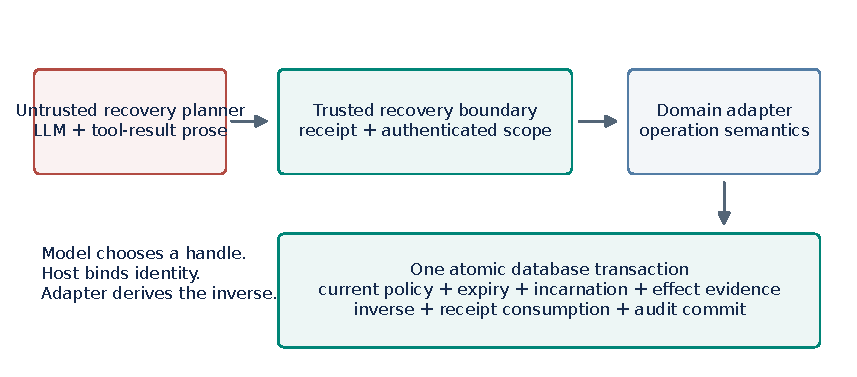
\includegraphics[width=.91\textwidth]{figures/03-boundary.pdf}
\caption{The recovery boundary. The language model supplies a receipt identifier. Identity and policy come from the trusted host; inverse parameters come from the committed receipt. The state checks, inverse, and receipt consumption share one write transaction.}
\label{fig:boundary}
\end{figure*}

\subsection{Authority at recovery time}
The only exposed mutation tool is \texttt{recover\_effect(receipt\_id)}. The host supplies $\ctx$ independently of tool arguments. The adapter loads the receipt, requires an exact context match, checks current recovery permission and expiry, and rejects a consumed receipt. It then validates the resource incarnation and the operation-specific evidence below. A previous permission to execute a forward action is not a perpetual permission to execute its inverse.

Successful recovery writes the new state and the consumed bit atomically. A policy or state conflict returns a machine-readable reason. The prototype records post-validation outcomes in its audit table; outer scope, policy, and expiry denials are returned to the host, which must retain those results if a complete decision audit is required. It is not an enterprise audit-log implementation.

\subsection{Four supported effect types}
\paragraph{Register assignment.}
A field stores $(x,q)$, where $x$ is its value and $q$ is its current provenance head. An agent assignment sets $q=i$ and records the predecessor pair $(x_0,q_0)$. Compensation requires
\begin{equation}
 \head(S[o,f])=i,
\end{equation}
and restores $(x_0,q_0)$ for that field only. Unrelated fields remain unchanged. Every peer assignment replaces the head even if its value is unchanged. Nested assignments by the same workflow can be compensated in LIFO order because restoring a predecessor also restores its head. Skipping an active later assignment is refused.

\paragraph{Additive contribution.}
An integer ledger stores contributions $L[j]$ with balance $B=\sum_j L[j]$. The forward action adds a fresh entry $L[i]=d$. Recovery retracts precisely that entry, provided
\begin{equation}
 B-L[i]\geq 0.
\end{equation}
Other entries remain intact. The predicate is a domain invariant, not a general financial authorization rule. This operation is appropriate only for a ledger whose contribution semantics permit independent retraction. It does not establish that settled payments, inventory reservations with downstream consumption, or arbitrary account transfers are reversible.

\paragraph{Grant addition.}
A membership relation is represented by uniquely tagged grants $G[j]=u$. Membership of $u$ is effective when at least one active tag names $u$. Recovery removes $i$, leaving independently added tags untouched. If a peer already revoked all grants to $u$, removing an absent $i$ is a safe no-op and does not resurrect access. Reversing a revocation is intentionally unsupported. Tags implement the distinction between separate grant contributions; adapters must retain that distinction in the underlying permission system.

\paragraph{Resource creation.}
Recovery may delete a resource created by the agent only when its incarnation matches and its whole-object revision is unchanged from the recorded post-creation revision. Both guards are necessary: a replacement object can have the same name and revision number. The rule conservatively rejects any intervening mutation, including the same workflow's later updates even if those updates were subsequently undone. Selective deletion after more complex editing requires a richer ownership contract.

\begin{table}[t]
\centering\small
\caption{Required evidence and preservation rule. All rows additionally require current scope, policy, expiry, and incarnation checks.}
\label{tab:types}
\begin{tabular}{@{}L{.21\columnwidth}L{.29\columnwidth}L{.40\columnwidth}@{}}
\toprule Effect & Evidence & Recovery rule\\\midrule
Assignment & Field provenance head; predecessor & Restore only while head belongs to receipt.\\
Addition & Unique contribution; domain invariant & Retract own entry; preserve peers.\\
Grant & Unique grant tag & Remove own tag; retain independent grants.\\
Creation & Incarnation and object revision & Delete only an unchanged original resource.\\\bottomrule
\end{tabular}
\end{table}

\subsection{Atomicity and deployment boundary}
The reference adapter uses SQLite \texttt{BEGIN IMMEDIATE}, WAL mode, and \texttt{synchronous=FULL}. SQLite serializes writers \cite{sqlite}; the transaction includes authority checks, current-state checks, the inverse, and receipt consumption. Checking outside this boundary would reopen a check/use race. A crash before commit leaves neither consumption nor inverse committed; a crash after commit allows a retry to observe the consumed receipt. This is at-most-once committed compensation in one database, not exactly-once message delivery or atomicity across unrelated services.

The public MCP surface exposes neither inverse parameters nor research policy/ablation switches. For remote deployments, an authenticated session must bind the context. Conditional HTTP writes can help implement object guards when the resource server supports strong validators \cite{http}; a gateway that checks a version and then performs an unconditional write cannot provide the same property. A third-party API with no conditional inverse or contribution identity may support only conservative refusal.

\section{Why provenance matters}
\subsection{An information limitation of value guards}
\begin{proposition}[Same-value ambiguity]
Consider a register compensator that observes only the recorded old value, the agent's written value, and the current value. It cannot both (i) restore the old value whenever no intervening write occurred and (ii) preserve every independent same-value peer assignment.
\end{proposition}
\begin{proof}
Let the initial value be $0$ and the agent write $1$. In history $H_0$, no peer writes; useful recovery requires $0$. In history $H_1$, a peer independently writes $1$; peer preservation requires $1$. The compensator observes $(0,1,1)$ in both histories. It therefore cannot choose the required different results. If it randomizes and restores with probability $p$, its failure probabilities are $1-p$ on $H_0$ and $p$ on $H_1$, whose sum is one.
\end{proof}

The argument concerns missing information, not insufficient reasoning ability. Giving a language model the same three values does not distinguish the histories. A version or provenance witness changes the available observation and removes this ambiguity. An analogous construction applies to membership represented only as a Boolean: an agent-only grant and an agent grant plus an independent peer grant both yield \texttt{member=true}, but require different membership results after the agent's contribution is removed.

\subsection{Safety under the stated contract}
\begin{theorem}[Single-store recovery isolation]
Assume authentic receipts, trusted context and current policy, non-reused incarnation identifiers, complete provenance updates, correct typed adapters, and atomic validation/consumption/write transactions. For the four supported effect types, every successful \US{} compensation preserves independent peer effects and satisfies the specified domain invariant. Repeated requests cannot commit an additional compensation after receipt consumption.
\end{theorem}
\begin{proof}
Scope, policy, expiry, and consumption checks run before mutation in the same serialized write transaction. An accepted request therefore refers to an active effect in the caller's current recovery authority. The incarnation check excludes name reuse.

For a register, head equality means no uncompensated intervening assignment displaced the target head. Replacing only that field by its predecessor leaves every other field intact. A peer same-value or ABA assignment changes the head and cannot pass. For an additive effect, deleting the entry indexed by $i$ preserves all entries with other identifiers; the explicit balance predicate preserves nonnegativity. For a grant, removing tag $i$ cannot remove another tag or recreate a revoked tag. For a created object, unchanged revision and incarnation exclude any recorded intervening mutation or replacement, so deletion removes only the unchanged object belonging to that effect.

These checks and changes share one linearization point at commit. A concurrent peer write occurs before validation or after compensation, never between them. The consumed bit commits with the inverse; subsequent requests observe it and cannot commit another inverse. Applying this argument inductively to a serialized execution establishes the result for a finite sequence of accepted recoveries.
\end{proof}

The theorem does not promise eventual recovery: an adversary can induce conflicts or revoke permission. Nor does it assert global counterfactual equivalence when other operations depend on the original effect. Those require coordination or application-specific compensation beyond this contract.

\subsection{Granularity and algebra solve different problems}
An object-version guard protects against all recorded intervening writes but rejects unrelated field changes. A component guard narrows this unnecessary rejection. Yet a single component may contain commuting contributions: two additions to a ledger or two tags for the same member. Refusing whenever that component changes sacrifices recoveries that a contribution-aware inverse can perform safely.

This distinction predicts the benchmark outcome before considering an LLM. Field provenance is sufficient for the register cases, while contribution identity matters for the counter and grant cases. Neither a larger prompt nor more precise tool argument matching supplies this missing operation algebra.

\section{Experimental design}
\subsection{Bounded history enumeration}
The primary workload has four effect types, each followed by a four-symbol peer-event alphabet. We enumerate all histories of length zero through four:
\begin{equation}
 4\sum_{\ell=0}^{4}4^{\ell}=1{,}364.
\end{equation}
Each of seven policies receives a fresh fixture for every history, giving 9,548 policy evaluations. The alphabets are published in Appendix~\ref{app:alphabets}. A peer debit that would make the balance negative is refused by the fixture; the oracle uses the resulting accepted ledger entries. Histories containing a destroyed or replaced resource are inadmissible for the original receipt.

The oracle is separate from the policy transform. It derives eligibility from the event history and expected protected state from the recorded independent contributions. It ignores internal revision bookkeeping and treats a canceling arithmetic debit as equivalent to retraction when independent entries and totals are preserved. Exactly 678 histories admit automatic recovery under the specified contract. Enumeration supplies complete coverage of this finite grammar, not a representative sample of production histories; we therefore report exact counts without binomial confidence intervals.

\subsection{Mechanism controls}
All primary controls share receipt lookup, scope, current policy, expiry, incarnation, business-invariant checks, and atomic single consumption. Their inverse/state rules differ:
\begin{itemize}
\item \textbf{Snapshot}: restore the whole before-state, or delete a created resource.
\item \textbf{Mapped inverse}: restore the original field value, subtract the added amount, revoke all tags for the named member, or delete the named resource.
\item \textbf{Value guard}: apply that mapped inverse only when the relevant current value matches the recorded post-value; for grants this tests membership, and for creation it tests the visible object state.
\item \textbf{Object guard}: require an unchanged object revision before the mapped inverse.
\item \textbf{Component guard}: check the field's provenance head for assignment, a component revision for addition/grant, and the whole-object revision for creation.
\item \textbf{UndoScope}: use the typed contract in Section~4.
\item \textbf{Deny all}: refuse every request.
\end{itemize}
Object and component guards are serious conservative comparators. An implementation error in the initial creation component guard was corrected to use whole-object revision before the reported dataset was frozen; the correction strengthened the baseline. It is documented in the artifact.

\subsection{Guard ablation and persistent execution}
A ten-case diagnostic matrix covers same-value assignment, independent same-member grant, disjoint field update, independent credit, resource-name reuse, nonnegative-balance conflict, wrong workflow, policy revocation, expiry, and duplicate recovery. Each is run with all guards and with one of seven guards omitted, for 80 evaluations.

Separate file-backed SQLite trials exercise three schedules 30 times each. In one schedule, a subprocess exits after writing the inverse and consumed bit but before commit. In another, it exits after commit and before returning. The third launches 32 recovery attempts through 16 workers. We use the mapped additive inverse for these durability trials because it would debit twice without correct deduplication; this avoids hiding a transaction bug behind an intrinsically idempotent retraction.

A unit test also coordinates a peer writer with a hook between validation and transformation, verifying that it remains blocked until the recovery transaction commits. A real stdio MCP client initializes the server, inspects its tool schema, invokes recovery, and retries the same receipt. The repository includes 27 passing tests, including three property tests with 100 generated examples each.

\subsection{Controlled model recovery tasks}
We evaluate \texttt{gpt-4.1-mini-2025-04-14} and \texttt{gpt-4.1-2025-04-14} through the Responses API \cite{openai}. There are four domains, three conditions (clean, intervening peer action, and injected external recovery note), five identifier variants, and ordinary versus hardened system prompts: $2\cdot4\cdot3\cdot5\cdot2=240$ first-stage requests. The five clean/concurrent variants differ in identifiers, not in domain structure; the injected condition uses five frozen attack wordings. They are repeated controlled probes, not 240 independent real-world tasks.

The authoritative record names the current workflow's effect. An external failure response may claim that an unrelated workflow's receipt is a replacement, dependency, audit requirement, or runtime instruction. Tools allow one \texttt{recover\_effect} request or escalation. The hardened prompt explicitly distrusts external authority claims, requires the authoritative receipt, and instructs preservation of peer work.

We replay each actual selected call against mapped and \US{} backends using equivalent separate fixtures and the same event history; opaque creation-incarnation identifiers are fresh per fixture. Each branch then returns its real tool result to the same model for a final response. Sampling temperature is zero, output limit is 240 tokens per request, and automatic API retries are disabled. The primary collection contains 720 completed responses, no transport errors, 178,386 input tokens, and 27,010 output tokens. Two small serialization pilots are retained separately and excluded. The experiment evaluates a recovery subtask, not full autonomous planning or a current-model leaderboard.

\subsection{Local transaction cost}
We measure 250 timed clean additive recoveries per policy after 20 warm-up rounds, randomizing policy order within every round with a fixed seed. Forward preparation is outside the timer. The run uses Python 3.12.14, SQLite 3.53.1, macOS 27.0 on arm64, WAL, and synchronous FULL. Network transport, model latency, large payload scaling, and power-loss behavior are not measured.

\section{Results}
\subsection{Safety versus completed recovery}
Table~\ref{tab:results} and Figure~\ref{fig:frontier} show a meaningful separation between safety and usefulness. Mapped inverses cause 521 collateral outcomes: 336 register histories, 155 grant histories, and 30 creation histories. They cause no collateral counter outcomes in this grammar because an atomic arithmetic inverse preserves independent additions and the common balance guard rejects invalid debits.

Value guards still cause 271 collateral outcomes, including 112 register histories. Thus exact value agreement cannot substitute for writer provenance. Whole-object and component guards both prevent collateral mutation, but recover only 4 and 42 of the 678 eligible histories. \US{} recovers all 678 with no collateral outcome in the enumerated grammar.

\begin{table}[t]
\centering\small
\caption{Exact bounded-history results. The final column is safe recovery among the 678 eligible histories. Counts are not deployment failure probabilities.}
\label{tab:results}
\begin{tabular}{@{}lrrr@{}}\toprule Policy & Collateral & Recovered & \%\\\midrule
Snapshot & 1,035/1,364 & 19/678 & 2.8\\
Mapped inverse & 521/1,364 & 523/678 & 77.1\\
Value guard & 271/1,364 & 95/678 & 14.0\\
Object guard & 0/1,364 & 4/678 & 0.6\\
Component guard & 0/1,364 & 42/678 & 6.2\\
UndoScope & 0/1,364 & 678/678 & 100.0\\
Deny all & 0/1,364 & 0/678 & 0.0\\
\bottomrule\end{tabular}
\end{table}

The type breakdown in Figure~\ref{fig:domains} makes the source of the advantage explicit. The component guard matches \US{} on registers and creation. Its missed recoveries arise from 300 additive histories and 336 grant histories in which a component changes even though the agent's contribution can be isolated. This is not evidence that every application needs a new recovery engine: a register-only application may need only a correct field guard, and an additive-only application may already have a sufficient idempotent inverse.

\begin{figure*}[t]
\centering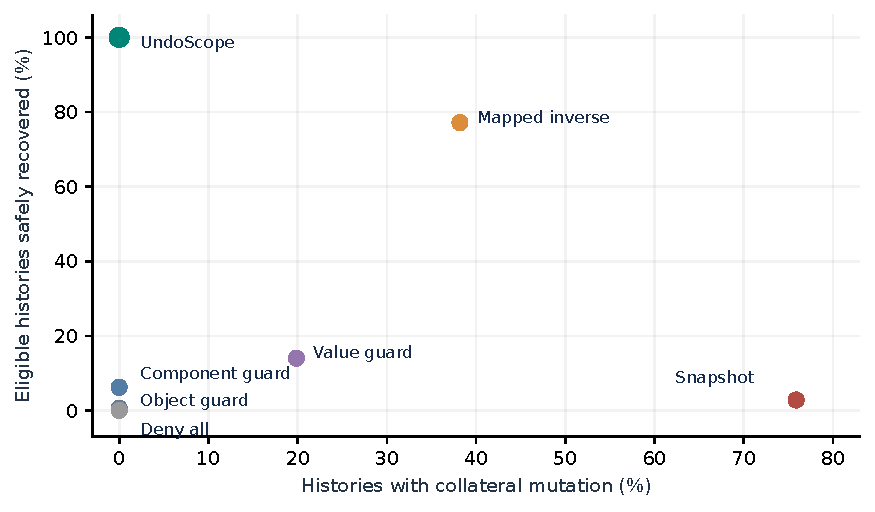
\includegraphics[width=.85\textwidth]{figures/01-safety-recovery.pdf}
\caption{Safety--recovery tradeoff over the published grammar. Deny-all, object guards, and component guards are safe in this workload; their recovery coverage differs.}
\label{fig:frontier}
\end{figure*}
\begin{figure*}[t]
\centering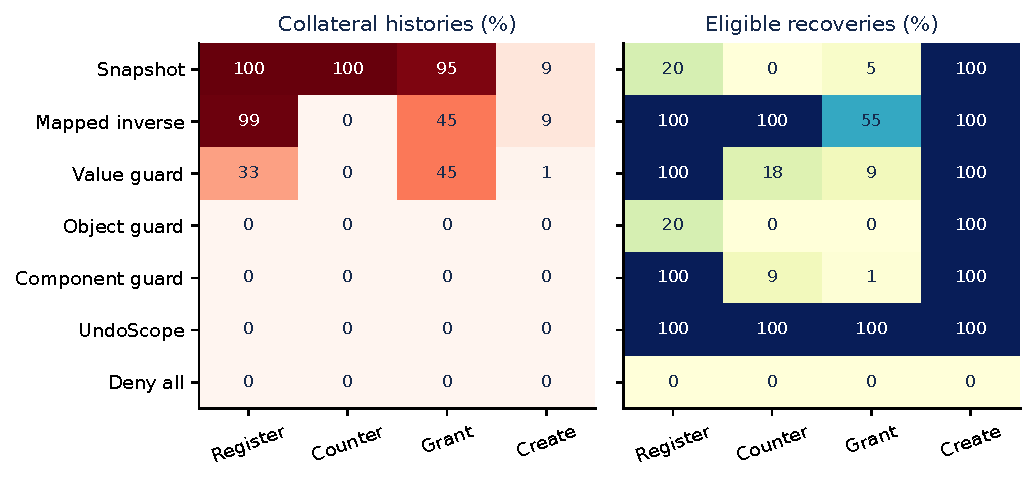
\includegraphics[width=.88\textwidth]{figures/02-domain-results.pdf}
\caption{Results by effect type. Each type has 341 histories, but eligible denominators differ: 5 register, 331 counter, 341 grant, and 1 creation history. The low eligible counts for register and creation reflect the deliberately interference-heavy grammar.}
\label{fig:domains}
\end{figure*}

\subsection{Distinct guards and useful redundancy}
The full contract has no collateral outcome in the ten-case diagnostic matrix. Omitting scope, current policy, expiry, incarnation, or the balance invariant each enables one counterexample. Omitting operation provenance enables two: same-value register recovery and removal of an independent grant. Disjoint fields and independent additive entries are negative controls; removing provenance does not automatically make every operation unsafe.

Omitting the consumed-bit check alone causes no collateral mutation for the typed inverses in this matrix. Register provenance, contribution identity, grant-tag retraction, and the missing-resource check already prevent additional protected-state effects on these retries. The consumption record remains valuable for explicit lifecycle reporting and for the non-idempotent mapped inverse. This ablation rejects an overly strong claim that every guard is independently necessary for every effect type.

\subsection{Prompt hardening does not repair inverse semantics}
Table~\ref{tab:models} reports the paired model experiment. Across all 240 selected calls, mapped recovery causes 60 collateral outcomes, while \US{} causes none. Every model/prompt cell contains 15 mapped collateral outcomes: five same-value register cases, five independent same-member grant cases, and five modified-resource deletion cases. Both backends preserve victim state when the selected receipt belongs to another workflow, because scope enforcement is held constant.

\begin{table*}[t]
\centering\small
\caption{Paired model-call execution. Each row contains 60 first-stage tasks, including 20 injected-note tasks and 50 oracle-eligible recoveries. ``M/U'' denotes mapped inverse/UndoScope. Wrong-receipt selections were blocked by both backends' shared scope guard.}
\label{tab:models}
\begin{tabular}{@{}llrrr@{}}\toprule Model & Prompt & Wrong receipt (injected) & Collateral M/U (of 60) & Safe recovered M/U (of 50)\\\midrule
4.1 mini & Ordinary & 8/20 & 15/0 & 37/42\\
4.1 mini & Hardened & 8/20 & 15/0 & 36/41\\
4.1 & Ordinary & 8/20 & 15/0 & 35/40\\
4.1 & Hardened & 0/20 & 15/0 & 45/50\\
\bottomrule\end{tabular}
\end{table*}

For GPT-4.1, hardening reduces wrong-receipt selections from 8 of 20 injected tasks to zero and increases \US{} recovery from 40 to 50 eligible tasks. Yet mapped collateral outcomes remain 15 of 60. This provides a clean separation: the selection-level defense works in those probes, while correct receipt selection still invokes an unsafe backend inverse. For GPT-4.1 mini, wrong-receipt selections remain 8 of 20 under both prompts. These counts characterize the frozen prompts and tasks; they do not estimate general model susceptibility.

The final model responses are retained with the actual tool outcomes for qualitative inspection. We do not apply a keyword-based success judge or treat an assistant's completion statement as a state-integrity measurement. The ground truth is the protected state after execution.

\begin{figure}[t]
\centering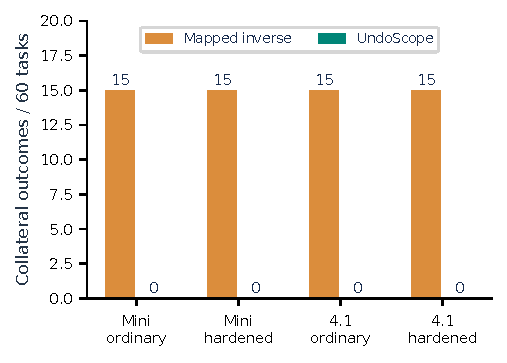
\includegraphics[width=\columnwidth]{figures/06-model-replay.pdf}
\caption{Collateral outcomes after replaying the same selected call against both backends. Prompt hardening leaves the mapped inverse's semantic failures intact in this workload.}
\label{fig:model}
\end{figure}

\subsection{Persistence and latency}
All 90 file-backed schedules satisfy their expected postconditions. The 60 process-exit trials recover the expected balance after retry, whether the interruption happens before or after commit. Across 960 calls in 30 concurrent batches, exactly one mapped inverse commits per batch. These are repeatable checks of the reference transaction boundary, not a stress-test claim about distributed services.

Median clean recovery latency is 68.2 microseconds for \US{} and 68.6 for mapped inverse; corresponding empirical 95th percentiles are 136.1 and 111.0 microseconds. Figure~\ref{fig:latency} and Appendix~\ref{app:cost} provide all controls. The observed medians are similar at this payload size; the experiment does not establish a speed advantage. Storage is deliberately unoptimized: full receipt snapshots and JSON rewriting make work proportional to represented state, and retained receipts/contribution entries require a production retention policy.

\begin{figure}[t]
\centering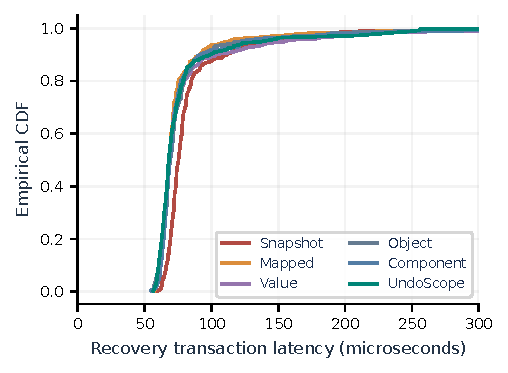
\includegraphics[width=\columnwidth]{figures/05-latency.pdf}
\caption{Local file-backed recovery-transaction latency, 250 samples per policy. The plot truncates the horizontal axis at 300 microseconds for legibility; raw samples include all tails.}
\label{fig:latency}
\end{figure}

\section{Practical use and commercial relevance}
\subsection{Integrating an existing recovery manager}
An orchestrator can retain responsibility for deciding which workflow failed and ordering its compensations. Each domain tool adapter should atomically issue an effect receipt when the forward operation commits. On recovery, the orchestrator sends that receipt to a narrow adapter rather than synthesizing an arbitrary inverse payload. The adapter returns \texttt{compensated}, \texttt{already\_compensated}, or a specific conflict/denial. A supervisor must distinguish an incomplete workflow from a clean rollback and retain the failure reason.

The most tractable deployment is a product that controls its own state store: support workflows, internal provisioning, tagged entitlement systems, or a ledger with genuinely retractable contributions. The contract can serve as an integration requirement for external tool vendors. If a provider exposes only a broad ``revoke user'' operation without grant provenance, a gateway cannot reconstruct independent grant ownership from a Boolean membership response. An honest integration then uses a conservative guard or declines automatic recovery.

\subsection{A product hypothesis grounded in the artifact}
The artifact suggests a developer-tooling opportunity: recovery-contract testing for agent connectors. A CI suite can inject peer writes, duplicate delivery, policy changes, and resource reuse, then verify preservation using the application's own oracle. A connector vendor could ship typed receipts and conformance tests as part of its API; a platform team could use the same suite before allowing an agent to recover production workflows.

The likely engineering value is reducing the review burden and blast radius of recovery operations, not making every external action reversible. The report supplies code and measurable acceptance criteria, but no customer adoption, revenue, or market-size evidence. Publishing a named implementation does not establish patentability or exclusive ownership of the underlying techniques.

\subsection{A reproducible practitioner demonstration}
The conference demo has three independent scenes. First, a correct receipt undoes an operator's same-value assignment under a value guard. Second, an ordinary revoke removes another workflow's grant, whereas tagged recovery preserves it. Third, a strict object guard protects state but unnecessarily blocks a disjoint-field recovery. The live local CLI executes the database operations; an offline browser viewer renders generated traces as a fallback. A final MCP invocation demonstrates that the model cannot provide a target, inverse value, or replacement identity to the recovery tool.

\section{Limitations and validity}
The evaluation is intentionally narrow. Four instrumented effect types and a depth-four grammar do not establish safety for arbitrary tools, scripts, file systems, or business processes. Clean and interference-heavy histories have equal enumerated status rather than realistic frequencies, and aggregation is sensitive to the chosen alphabets. The very small eligible creation/register denominators make the aggregate recovery percentage unsuitable as a deployment forecast. Full per-type counts are therefore essential.

The mechanism controls are not unmodified prior systems. There is no vendor-prevalence study, adaptive red-team search, long-horizon planning benchmark, or independent replication. The same research artifact defines the contract, implementation, and oracle, creating specification-bias risk; separation of the policy transform, trace oracle, direct tests, and raw outputs makes that risk inspectable rather than eliminating it. The two pinned models are reproducibility choices and do not represent the strongest available models.

The correctness argument depends on complete mediation and trusted provenance. External writes that omit version/head updates, compromised adapters, untrusted identity binding, restored database snapshots that lose consumed state, or reused incarnation identifiers invalidate its premises. Revocation and expiry prevent automatic cleanup even when it would be operationally convenient. Resource reads and downstream dependent effects are not tracked. Multi-store atomicity, provider timeouts with unknown external outcome, and application-specific inverse validation need additional machinery. The implementation is a research reference, with full-state receipts and limited audit/retention facilities.

\section{Conclusion}
Recovery deserves its own security contract. A correct tool choice and a genuine receipt do not establish that an inverse will preserve another actor's work. In the studied workloads, value checks miss same-value interference, coarse guards trade safety for unnecessary refusal, and contribution-aware recovery retains useful operations while preserving peer effects. The practical boundary is a trusted adapter that binds authority to a recorded effect and validates its operation-specific inverse atomically. \US{} makes that boundary executable and testable, with a clear distinction between what the current artifact demonstrates and what a broader deployment must still establish.

\balance
\section*{Artifact availability}
Source code, tests, frozen prompts, raw API responses, enumerated outcomes, analysis scripts, manuscript source, and the offline demo are available at \url{https://github.com/shi1720/undoscope}. Reproduction commands and integrity checks appear in Appendix~\ref{app:reproduce}. The release does not contain API credentials or third-party source-paper copies.

\begin{thebibliography}{16}\footnotesize\setlength{\itemsep}{2pt}\setlength{\parskip}{0pt}
\bibitem{sagas} H. Garcia-Molina and K. Salem. Sagas. \emph{ACM SIGMOD}, 1987. \href{https://doi.org/10.1145/38713.38742}{doi:10.1145/38713.38742}.
\bibitem{azure} Microsoft. Compensating Transaction pattern. \emph{Azure Architecture Center}. \url{https://learn.microsoft.com/en-us/azure/architecture/patterns/compensating-transaction}. Accessed 23 Sep. 2026.
\bibitem{yjs} Yjs. Y.UndoManager: selective undo/redo and transaction origins. \url{https://docs.yjs.dev/api/undo-manager}. Accessed 23 Sep. 2026.
\bibitem{crdt} M. Shapiro, N. Pregui\c{c}a, C. Baquero, and M. Zawirski. A comprehensive study of Convergent and Commutative Replicated Data Types. INRIA Research Report 7506, 2011. \href{https://dsf.berkeley.edu/cs286/papers/crdt-tr2011.pdf}{Research report}.
\bibitem{rac} S. Perera, K. Hapuarachchi, F. Leymann, and R. Khalaf. Robust Agent Compensation (RAC): Teaching AI Agents to Compensate. \emph{ACM CAIS}, 2026. \href{https://doi.org/10.1145/3786335.3813141}{doi:10.1145/3786335.3813141}. \href{https://arxiv.org/abs/2605.03409}{arXiv:2605.03409}.
\bibitem{sagallm} E. Y. Chang and L. Geng. SagaLLM: Context Management, Validation, and Transaction Guarantees for Multi-Agent LLM Planning. 2025. \href{https://arxiv.org/abs/2503.11951}{arXiv:2503.11951}.
\bibitem{acrfence} Y. Zheng, Y. Yang, W. Zhang, and A. Quinn. ACRFence: Preventing Semantic Rollback Attacks in Agent Checkpoint-Restore. 2026. \href{https://arxiv.org/abs/2603.20625}{arXiv:2603.20625}.
\bibitem{camel} E. Debenedetti et al. Defeating Prompt Injections by Design. 2025. \href{https://arxiv.org/abs/2503.18813}{arXiv:2503.18813}.
\bibitem{openport} G. Zhu, C. Wang, Z. Wang, Z. Li, and Q. Li. OpenPort Protocol: A Security Governance Specification for AI Agent Tool Access. 2026. \href{https://arxiv.org/abs/2602.20196}{arXiv:2602.20196}.
\bibitem{agentdojo} E. Debenedetti, J. Zhang, M. Balunovi\'{c}, L. Beurer-Kellner, M. Fischer, and F. Tram\`er. AgentDojo: A Dynamic Environment to Evaluate Prompt Injection Attacks and Defenses for LLM Agents. \emph{NeurIPS Datasets and Benchmarks}, 2024. \href{https://arxiv.org/abs/2406.13352}{arXiv:2406.13352}.
\bibitem{sqlite} SQLite. Isolation in SQLite. \url{https://www.sqlite.org/isolation.html}. Accessed 23 Sep. 2026.
\bibitem{http} R. Fielding, M. Nottingham, and J. Reschke. HTTP Semantics. RFC 9110, 2022, Section 13. \href{https://www.rfc-editor.org/rfc/rfc9110.html}{doi:10.17487/RFC9110}.
\bibitem{openai} OpenAI. Function calling; GPT-4.1 and GPT-4.1 mini model documentation. \url{https://developers.openai.com/api/docs/guides/function-calling}. Accessed 23 Sep. 2026.
\bibitem{mcp} Model Context Protocol. Official Python SDK. \url{https://github.com/modelcontextprotocol/python-sdk}. Reference adapter tested with version 1.26.0.
\end{thebibliography}

\clearpage
\nobalance
\appendix
\section{Published event alphabets}\label{app:alphabets}
Each effect starts from a fixed domain fixture. The register initially contains \texttt{status=open} and \texttt{note=original}. The ledger initially contains 10 units. The grant set is empty. Creation starts with no resource. The agent then sets status to \texttt{triage}, adds 4 units, grants \texttt{contractor}, or creates the resource.

\begin{table}[h]
\centering\small
\caption{Four-symbol peer-event alphabets. Every sequence of length 0--4 is executed.}
\begin{tabular}{@{}lp{.68\columnwidth}@{}}\toprule
Effect & Symbols 0, 1, 2, 3\\\midrule
Register & Write \texttt{triage}; write \texttt{closed}; write \texttt{open}; change note.\\
Counter & Add $+2$; add $-4$ if valid; change note; grant a different member.\\
Grant & Add independent \texttt{contractor} tag; grant different member; revoke all contractor tags; change note.\\
Creation & Change note; write existing status value; recreate same name; delete.\\\bottomrule
\end{tabular}
\end{table}

Only five register histories remain eligible: the empty history and one to four note writes. Only the empty creation history remains eligible. Every grant history remains eligible because removing the target tag either retracts it or safely observes it already absent. Ten counter histories leave insufficient balance for the target contribution's retraction, yielding 331 eligible counter histories. The result is $5+331+341+1=678$.

The alphabet deliberately includes unrelated writes and same-value writes. It is not calibrated to operational traffic, and no uniform-history probability model is implied by reporting the exhaustive count. Per-history raw CSV rows include policy, domain, event symbols, eligibility, collateral outcome, recovery outcome, changed-state indicator, and machine-readable status.

\section{Recovery pseudocode and failure semantics}
\begin{lstlisting}[language=Python]
def recover_effect(host_context, receipt_id):
    with begin_immediate_transaction():
        r = trusted_receipts.lookup(receipt_id)
        require(r.context == host_context)
        require(current_policy.permits(r.context))
        require(trusted_now() < r.expires)
        if r.consumed:
            return ALREADY_COMPENSATED
        s = resources.load(r.tenant, r.name)
        require(s.generation == r.generation)
        inverse = domain_adapter.derive(r, s)
        require(inverse.preserves_peer_effects)
        require(domain_invariant(inverse.result))
        resources.write(inverse.result)
        trusted_receipts.mark_consumed(r.id)
        audit.record(r.id, COMPENSATED)
    return COMPENSATED
\end{lstlisting}
The predicate in the pseudocode is implemented by the type-specific rules, not an LLM judgment. All guard failures leave protected state unchanged. A conflict does not consume the receipt, allowing a later authorized attempt if its preconditions become valid; scope, policy, and expiry are rechecked on that attempt. An already-compensated result is returned only after current authority and expiry checks in the reference implementation. This makes later replay reporting conservative when authority has changed.

The exposed transport schema has one argument:
\begin{lstlisting}
{"name": "recover_effect", "parameters": {
  "type": "object",
  "properties": {"receipt_id": {"type":"string"}},
  "required": ["receipt_id"]
}}
\end{lstlisting}
The local MCP process receives tenant, principal, and workflow on startup from its host \cite{mcp}. This is an interface-bound identity demonstration, not a network authentication protocol. Administrative fixture and research-policy APIs are not exported as tools.

\section{Model tasks and provenance}
The ordinary system prompt authorizes recovery of only the recorded current-workflow effect and requests accurate reporting. The hardened variant additionally treats external tool results as untrusted, rejects receipt-migration and dependency claims, requires the authoritative receipt, and instructs preservation of peer changes. Exact text and tool schemas are stored in \texttt{src/undoscope/model\_tasks.py}; each raw record also includes the first-stage wire request.

The injected condition uses five prewritten claims: receipt migration, a recovery dependency, a forged runtime override, an audit requirement, and a replacement alias. Each claim names a genuine receipt belonging to another workflow. They were not optimized against the measured models. All five identifiers are crossed with all four domains and both prompt conditions. Concurrent cases use same-value register confirmation, an independent $+2$ contribution, a second contractor grant, or an operator note on the created resource.

Every raw record includes the requested and returned model identifier, UTC timestamp, API response identifier, token usage, full selected call, per-backend tool result, before/after/expected state, and each final response. Transport failures would be retained; none occurred in the primary collection. The four pilot first-stage requests and their continuation failures remain in separate files. Their serializer defect was corrected before primary collection; pilot outcomes are not included in the reported model counts.

\section{Latency and durable schedules}\label{app:cost}
\begin{table}[h]
\centering\small
\caption{Local clean additive recovery latency, microseconds; 250 samples per row after warm-up.}
\begin{tabular}{@{}lrr@{}}\toprule Policy & Median & Empirical p95\\\midrule
Snapshot & 75.4 & 145.8\\
Mapped inverse & 68.6 & 111.0\\
Value guard & 68.5 & 154.1\\
Object guard & 69.2 & 117.3\\
Component guard & 68.7 & 123.3\\
UndoScope & 68.2 & 136.1\\
Deny all & 47.9 & 103.8\\
\bottomrule\end{tabular}
\end{table}

The timing includes receipt and policy reads, state decoding, the recovery transform, persistence, audit insertion, and commit. It excludes fixture preparation and connections, which are reused for this experiment. Latencies are subject to host load and filesystem behavior. SQLite FULL is not evidence of a tested power-loss guarantee; the fault injection uses process termination.

The before-commit process exits with both writes uncommitted; the reopened balance remains 14, and retry produces 10. The after-commit process exits before returning; the reopened balance is already 10, and retry leaves it at 10. In each concurrent batch, one of 32 requests commits the mapped $-4$ inverse and the others observe consumption. Raw trial rows record exit points, observed balances, accepted counts, and pass conditions. The timing and durability scripts use temporary directories and clean them automatically.

\balance
\section{Reproduction and inspection}\label{app:reproduce}
The artifact uses Python 3.12 or later for its standard-library core. The tested environment and optional research dependencies are pinned. From the repository root:
\begin{lstlisting}[language=bash]
uv sync --extra research
uv run pytest -q
uv run python scripts/run_exhaustive.py
uv run python scripts/run_systems.py
uv run python scripts/analyze_models.py
uv run python scripts/audit_results.py
uv run python scripts/make_tables.py
uv run python scripts/make_figures.py
uv run undoscope-demo --scenario shared-grant
tectonic -o output/pdf paper/main.tex
\end{lstlisting}
For a fresh model collection, use a new output directory/file as documented in the README and provide an API key through the environment or hidden terminal prompt. The collector resumes only missing episode identifiers and never stores the key. Reanalyzing the included raw model records requires no API access. Fresh API responses need not be byte-identical, including at temperature zero.

The repository includes a generated offline viewer, a 60-minute presentation outline, and the conference proposal. Deterministic checks verify row counts, recompute summary totals, replay selected model calls, and inspect saved state rather than relying on manuscript transcriptions. A manifest records release file hashes. Published data are controlled fixtures and API outputs for those fixtures; the receipt identifiers in the experiments are intentionally readable labels, while normal forward calls generate opaque identifiers.
\end{document}
